\let\negmedspace\undefined
\let\negthickspace\undefined
\documentclass[journal]{IEEEtran}
\usepackage[a5paper, margin=10mm, onecolumn]{geometry}
\usepackage{lmodern} % Ensure lmodern is loaded for pdflatex
\usepackage{tfrupee} % Include tfrupee package

\setlength{\headheight}{1cm} % Set the height of the header box
\setlength{\headsep}{0mm}     % Set the distance between the header box and the top of the text

\usepackage{gvv-book}
\usepackage{gvv}
\usepackage{cite}
\usepackage{amsmath,amssymb,amsfonts,amsthm}
\usepackage{algorithmic}
\usepackage{graphicx}
\usepackage{textcomp}
\usepackage{xcolor}
\usepackage{txfonts}
\usepackage{listings}
\usepackage{enumitem}
\usepackage{mathtools}
\usepackage{gensymb}
\usepackage{comment}
\usepackage[breaklinks=true]{hyperref}
\usepackage{tkz-euclide} 
\usepackage{listings}                                      
\def\inputGnumericTable{}                                 
\usepackage[latin1]{inputenc}                                
\usepackage{color}                                            
\usepackage{array}                                            
\usepackage{longtable}
\usepackage{multicol}
\usepackage{calc}                                             
\usepackage{multirow}                                         
\usepackage{hhline}                                           
\usepackage{ifthen}                                           
\usepackage{lscape}
\begin{document}

\bibliographystyle{IEEEtran}
\vspace{3cm}

\title{12.8.3.9}
\author{EE24BTECH11011- Pranay Kumar}
% \maketitle
% \newpage
% \bigskip
{\let\newpage\relax\maketitle}

\renewcommand{\thefigure}{\theenumi}
\renewcommand{\thetable}{\theenumi}
\setlength{\intextsep}{10pt} % Space between text and floats


\numberwithin{equation}{enumi}
\numberwithin{figure}{enumi}
\renewcommand{\thetable}{\theenumi}


\textbf{Question}:\newline
Find the area of the smaller region bounded by the ellipse $\frac{x^2}{25} + \frac{y^2}{9} = 1$ and the line $\frac{x}{5} + \frac{y}{3} = 1$

Theoretical Solution:\\
The point of intersection of the line with the ellipse is $x_i=h+k_i m$,\\
where,$k_i$ is a constant and is calculated as follows:-
$$k_i=\frac{1}{m^\top Vm}\brak{-m^\top \brak{Vh+u}\pm \sqrt{\sbrak{m^\top \brak{Vh+u}}^2-g\brak{h}\brak{m^\top Vm}}}$$\\
Substituting the input parameters in $k_i$,\\
\begin{multline}
     k_i =\frac{1}{\myvec{\frac{1}{b}&\frac{-1}{a}}\myvec{b^2&0\\0&a^2}\myvec{\frac{1}{b}\\\frac{-1}{a}}}\brak{-\myvec{\frac{1}{b}&\frac{-1}{a}}\brak{\myvec{b^2&0\\0&a^2}\myvec{a\\0}+\myvec{0\\0}}\pm \\
     \sqrt{\sbrak{\myvec{\frac{1}{b}&\frac{-1}{a}}\brak{\myvec{b^2&0\\0&a^2}\myvec{a\\0}+\myvec{0\\0}}}^2-g\brak{h}\brak{\myvec{\frac{1}{b}&\frac{-1}{a}}\myvec{b^2&0\\0&a^2}\myvec{\frac{1}{b}\\\frac{-1}{a}}}}} 
\end{multline}
We get,\\
$$k_i= 0,-ab$$
Substituting $k_i$ in $x_i=h+k_i m$  we get,\\
\begin{align}
     x_1&=\myvec{a\\0}+\brak{0}\myvec{\frac{1}{b}\\\frac{-1}{a}}\\
    \implies x_1 &=\myvec{a\\0}\\
    x_2 &=\myvec{a\\0}+\brak{-ab}\myvec{\frac{1}{b}\\\frac{-1}{a}}\\
    \implies x_2&=\myvec{a\\0}+\myvec{-a\\b}\\
    \implies x_2&=\myvec{0\\b}
\end{align}
The area of the smaller region bounded by the ellipse $\frac{x^2}{25} + \frac{y^2}{9} = 1$ and the line $\frac{x}{5} + \frac{y}{3} = 1$ is
\begin{align}
    &=\int_{0}^{a} \frac{b}{a}\sqrt{a^2-x^2} \,dx-\int_{0}^{a} \frac{b}{a}\brak{a-x} \,dx\\
    &=\frac{b}{a}\brak{\frac{x}{2}\sqrt{a^2-x^2}+\frac{a^2}{2}\sin^{-1}{\frac{x}{a}}-ax+\frac{x^2}{2}}\limits_{0}^{a}\\
    &=\frac{b}{a}\brak{\frac{\pi a^2}{4}-\frac{a^2}{2}}=\frac{ab}{2}\brak{\frac{\pi}{2}-1}
\end{align}
The given area is $\frac{ab}{2}\brak{\frac{\pi}{2}-1}$ sq. units\\
$\therefore$ Upon substituting $a=5,b=3$ the given area is $5\brak{\frac{\pi}{2}-1}\text{sq. units}\approx2.712$ sq. units\\
\newline
Computational Solution:\\
Using the Trapezoidal rule which approximates the integral of a function $f\brak{x}$ over an interval $\sbrak{a,b}$ by dividing the interval into $n$ subintervals and approximating the area under the curve as a series of trapezoids
\begin{align}
    \int_a^b f\brak{x}dx\approx\frac{h}{2}\sbrak{f\brak{x_0}+2\sum_{i=1}^{n-1}\brak{f\brak{x_i}+f\brak{x_n}}}
\end{align}
Where $x_0$ is semi-major axis of ellipse and $x_n$ is semi-minor axis of the ellipse and $h$ is the width of each subinterval.
\begin{align}
    x_n=x_0+n\cdot h\\
    \implies h=\frac{x_n-x_0}{n}
\end{align}
In the case of our problem of the area between the line and ellipse the area is computed by:
\begin{align}
    A=\int_{x_{0}}^{x_{n}}\brak{f_{ellipse}\brak{x}-f_{line}\brak{x}}dx\\
    f_{ellipse}\brak{x}=\sqrt{9\brak{1-\frac{x^2}{25}}}\\
    f_{line}\brak{x}=3-\frac{3x}{5}
\end{align}
Where $\sbrak{x_{0},x_{n}}$ are the intersection points. We need to find the area of $y_x$ from $x_0$ to $x_n$. Taking trapezoids of small width $h$ and discretizing points on the $x$ axis $x_0, x_1, x_2, \dots, x_n$. The sum of the trapezoidal areas will be
\begin{align}
    A&=\frac{1}{2}h\brak{y\brak{x_1}+y\brak{x_0}}+ \frac{1}{2}h\brak{y\brak{x_2}+y\brak{x_1}}+\dots+\frac{1}{2}h\brak{y\brak{x_n}+y\brak{x_{n-1}}}\\
  &=h\sbrak{\frac{1}{2}\brak{y\brak{x_0}+y\brak{x_n}}+ y\brak{x_1}+\dots+y\brak{x_{n-1}}}
\end{align}
Let $A\brak{x_n}$ be the area enclosed by the curve $y\brak{x}$ from $x=x_0$ to $x=x_n$, $\brak{x_0, x_1, \dots x_n}$ be equidistant points with step-size $h$.
\begin{align}
  A\brak{x_n+h}=A\brak{x_n}+\frac{1}{2}h\brak{y\brak{x_n+h}+y\brak{x_n}}
\end{align}
We can repeat this till we get the required area.\\
Discretizing the steps, making $A\brak{x_n}=A_n, y\brak{x_n}=y_n$ we get,
\begin{align}
 A_{n+1}=A_n+\frac{1}{2}h\brak{y_{n+1}+y_n}
\end{align}
We can write $y_{n+1}$ in terms of $y_n$ using the first principle of derivative. $y_{n+1}=y_n+hy^{\prime}_n$
\begin{align}
  A_{n+1}&=A_n+\frac{1}{2}h\brak{y_{n+1}+y_n}
\end{align}
We can write $y_{n+1}$ in terms of $y_n$ using the first principle of derivative. $y_{n+1}=y_n+hy^{\prime}_n$
\begin{align}
  A_{n+1}&=A_n+\frac{1}{2}h\brak{\brak{y_n+hy^{\prime}_n}+y_n}\\
  A_{n+1}&=A_n+\frac{1}{2}h\brak{2y_n+hy^{\prime}_n}\\
  A_{n+1}&=A_n+hy_n+\frac{1}{2}h^2y^{\prime}_n\\
  x_{n+1}&=x_n+h
\end{align}

In the given question, $y_n=\sqrt{9\brak{1-\frac{x_n^2}{25}}}+\frac{3x_n}{5}-3$ and $y^{\prime}_n=\frac{3}{5}\brak{1-\frac{x_n}{\sqrt{25-x^2}}}$\\
General Difference Equation will be given by,
\begin{align}
  A_{n+1}&=A_n+hy_n+\frac{1}{2}h^2y^{\prime}_n\\
  &=A_n+h\brak{\sqrt{9\brak{1-\frac{x_n^2}{25}}}+\frac{3x_n}{5}-3}+\frac{1}{2}h^2\brak{\frac{3}{5}\brak{1-\frac{x_n}{\sqrt{25-x^2}}}}\\
  x_{n+1}&=x_n+h
\end{align}
Iterating till we reach $x_n=5$ will return the required area.\\
Area obtained computationally: $2.7123332003665432$ sq. units\\
Area obtained theoretically: $5\brak{\frac{\pi}{2}-1}=2.71238898038$ sq. units.\\
As $n$ tends to infinity $A_n$ will be the exact area of the ellipse.
\begin{figure}[h!]
   \centering
   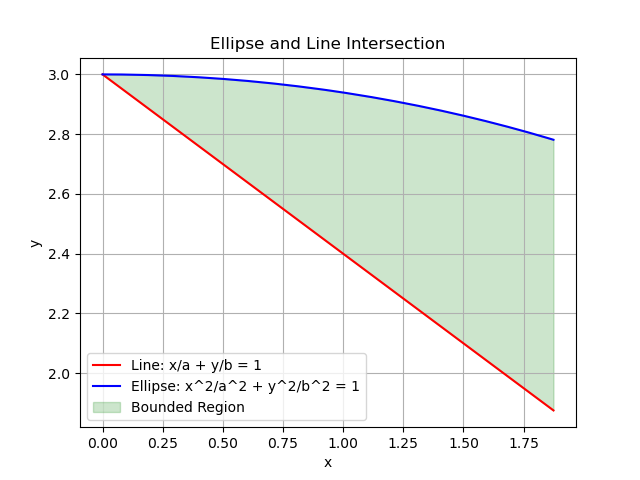
\includegraphics[width=1\linewidth]{figs/fig.png}
   
   \label{stemplot}
\end{figure}
\end{document}

